%%%%%%%%%%%%%%%%%%%%%%%%%%%%%%%%%%%%%%%%%
% Masters/Doctoral Thesis 
% LaTeX Template
% Version 2.5 (27/8/17)
%
% This template was downloaded from:
% http://www.LaTeXTemplates.com
%
% Version 2.x major modifications by:
% Vel (vel@latextemplates.com)
%
% This template is based on a template by:
% Steve Gunn (http://users.ecs.soton.ac.uk/srg/softwaretools/document/templates/)
% Sunil Patel (http://www.sunilpatel.co.uk/thesis-template/)
%
% Template license:
% CC BY-NC-SA 3.0 (http://creativecommons.org/licenses/by-nc-sa/3.0/)
%
%%%%%%%%%%%%%%%%%%%%%%%%%%%%%%%%%%%%%%%%%

%----------------------------------------------------------------------------------------
%	PACKAGES AND OTHER DOCUMENT CONFIGURATIONS
%----------------------------------------------------------------------------------------

\documentclass[
11pt, % The default document font size, options: 10pt, 11pt, 12pt
oneside, % Two side (alternating margins) for binding by default, uncomment to switch to one side
english, % ngerman for German
singlespacing, % Single line spacing, alternatives: onehalfspacing or doublespacing
%draft, % Uncomment to enable draft mode (no pictures, no links, overfull hboxes indicated)
%nolistspacing, % If the document is onehalfspacing or doublespacing, uncomment this to set spacing in lists to single
%liststotoc, % Uncomment to add the list of figures/tables/etc to the table of contents
%toctotoc, % Uncomment to add the main table of contents to the table of contents
%parskip, % Uncomment to add space between paragraphs
%nohyperref, % Uncomment to not load the hyperref package
headsepline, % Uncomment to get a line under the header
%chapterinoneline, % Uncomment to place the chapter title next to the number on one line
%consistentlayout, % Uncomment to change the layout of the declaration, abstract and acknowledgements pages to match the default layout
]{MastersDoctoralThesis} % The class file specifying the document structure

\usepackage[utf8]{inputenc} % Required for inputting international characters
\usepackage[T1]{fontenc} % Output font encoding for international characters

\usepackage{mathpazo} % Use the Palatino font by default

\usepackage[backend=bibtex]{biblatex} % Use the bibtex backend with the authoryear citation style (which resembles APA)

\addbibresource{assig1.bib} % The filename of the bibliography

\usepackage[autostyle=true]{csquotes} % Required to generate language-dependent quotes in the bibliography

%----------------------------------------------------------------------------------------
%	MARGIN SETTINGS
%----------------------------------------------------------------------------------------

\geometry{
	paper=a4paper, % Change to letterpaper for US letter
	inner=2.5cm, % Inner margin
	outer=3.8cm, % Outer margin
	bindingoffset=.5cm, % Binding offset
	top=1.5cm, % Top margin
	bottom=1.5cm, % Bottom margin
	%showframe, % Uncomment to show how the type block is set on the page
}

%----------------------------------------------------------------------------------------
%	THESIS INFORMATION
%----------------------------------------------------------------------------------------

\thesistitle{Deliverable 1: Context and scope of the project} % Your thesis title, this is used in the title and abstract, print it elsewhere with \ttitle
\supervisor{Dr. Jordi \textsc{Cortadella}} % Your supervisor's name, this is used in the title page, print it elsewhere with \supname
\examiner{} % Your examiner's name, this is not currently used anywhere in the template, print it elsewhere with \examname
\degree{Computer Science Degree} % Your degree name, this is used in the title page and abstract, print it elsewhere with \degreename
\author{Marc \textsc{Benedí}} % Your name, this is used in the title page and abstract, print it elsewhere with \authorname
\addresses{} % Your address, this is not currently used anywhere in the template, print it elsewhere with \addressname

\subject{} % Your subject area, this is not currently used anywhere in the template, print it elsewhere with \subjectname
\keywords{} % Keywords for your thesis, this is not currently used anywhere in the template, print it elsewhere with \keywordnames
\university{\href{https://www.upc.edu/ca}{Universitat Politècnica de Catalunya}} % Your university's name and URL, this is used in the title page and abstract, print it elsewhere with \univname
\department{\href{https://www.fib.upc.edu/ca/recerca/departaments/ciencies-de-la-computacio}{Department of Computer Science}} % Your department's name and URL, this is used in the title page and abstract, print it elsewhere with \deptname
\group{\href{}{}} % Your research group's name and URL, this is used in the title page, print it elsewhere with \groupname
\faculty{\href{https://www.google.co.uk/search?ei=y0GXWteBJsXSwQLJ8IGIDA&q=fib&oq=fib&gs_l=psy-ab.3..35i39k1l2j0i67k1j0l7.1898.2078.0.2162.3.3.0.0.0.0.92.172.2.2.0....0...1.1.64.psy-ab..1.2.172....0.Ha_7J3E1vcI}{Facultat Informàtica de Barcelona}} % Your faculty's name and URL, this is used in the title page and abstract, print it elsewhere with \facname

\newcommand{\projectTitle}{Design of an environment for solving pseudo-boolean optimization problems}
\newcommand{\courseName}{GEP}
\newcommand{\city}{Edinburgh, UK}

\AtBeginDocument{
\hypersetup{pdftitle=\ttitle} % Set the PDF's title to your title
\hypersetup{pdfauthor=\authorname} % Set the PDF's author to your name
\hypersetup{pdfkeywords=\keywordnames} % Set the PDF's keywords to your keywords
}

\begin{document}

\frontmatter % Use roman page numbering style (i, ii, iii, iv...) for the pre-content pages

\pagestyle{plain} % Default to the plain heading style until the thesis style is called for the body content

%----------------------------------------------------------------------------------------
%	TITLE PAGE
%----------------------------------------------------------------------------------------

\begin{titlepage}
\begin{center}

\vspace*{.06\textheight}
{\scshape\LARGE \univname\par}\vspace{1.5cm} % University name
\textsc{\Large \ttitle}\\[0.5cm] % Thesis type

\HRule \\[0.4cm] % Horizontal line
{\huge \bfseries \projectTitle\par}\vspace{0.4cm} % Thesis title
\HRule \\[1.5cm] % Horizontal line
 
\begin{minipage}[t]{0.4\textwidth}
\begin{flushleft} \large
\emph{Author:}\\
\href{https://marcb.pro}{\authorname} % Author name - remove the \href bracket to remove the link
\end{flushleft}
\end{minipage}
\begin{minipage}[t]{0.4\textwidth}
\begin{flushright} \large
\emph{Supervisor:} \\
\href{https://www.cs.upc.edu/~jordicf/}{\supname} % Supervisor name - remove the \href bracket to remove the link  
\end{flushright}
\end{minipage}\\[3cm]
 
\vfill

\large \textit{ }\\[0.3cm] % University requirement text
\textit{ }\\[0.4cm]
%\groupname\\\deptname\\[2cm] % Research group name and department name
\courseName\\[2cm]
\vfill

{\large \today \\ \city}\\[4cm] % Date
%
\includegraphics{UPCLogo.png} % University/department logo - uncomment to place it
 
\vfill
\end{center}
\end{titlepage}

%----------------------------------------------------------------------------------------
%	ABSTRACT PAGE
%----------------------------------------------------------------------------------------

%\begin{abstract}
%	\addchaptertocentry{\abstractname} % Add the abstract to the table of contents
%	In this deliverable, a first introduction into the project context\ref{Chapter1} will be made. \emph{Boolean Satisfiability Problems} are explained together with other important concepts for this project like \emph{Boolean Formula, Pseudo-Boolean Formula, Conjunctive Normal Form, Minimization, \ldots} The background for this project and motivations will also be detailed. \\
%	Next, the Project Formulation\ref{Chapter2} will be exposed, where the general objectives of it will be defined. \\
%	Later, the Scope\ref{Chapter3} of the project will be discussed together with what requirements the project should meet, how are they going to be made and what obstacles could be found.\\
%	Finally, the used methodology, the tools and the rigor will be exposed in Methodology and Rigor\ref{Chapter4}.
	
%\end{abstract}

%----------------------------------------------------------------------------------------
%	GLOSSARY
%----------------------------------------------------------------------------------------

%\begin{abbreviations}{ll} % Include a list of abbreviations (a table of two columns)
	
%	\textbf{LAH} & \textbf{L}ist \textbf{A}bbreviations \textbf{H}ere\\
%	\textbf{WSF} & \textbf{W}hat (it) \textbf{S}tands \textbf{F}or\\
%	bdd, cnf, sat ,boolean formula, pseudo boolean formula, minimization, modelo, interpretacion
	
%\end{abbreviations}

%----------------------------------------------------------------------------------------
%	LIST OF CONTENTS/FIGURES/TABLES PAGES
%----------------------------------------------------------------------------------------

\tableofcontents % Prints the main table of contents

%\listoffigures % Prints the list of figures

%\listoftables % Prints the list of tables

%----------------------------------------------------------------------------------------
%	THESIS CONTENT - CHAPTERS
%----------------------------------------------------------------------------------------

\mainmatter % Begin numeric (1,2,3...) page numbering

\pagestyle{thesis} % Return the page headers back to the "thesis" style

% Include the chapters of the thesis as separate files from the Chapters folder
% Uncomment the lines as you write the chapters

\chapter{Introduction and Sate-of-art} % Main chapter title

\label{Chapter1} % Change X to a consecutive number; for referencing this chapter elsewhere, use \ref{ChapterX}

\section{Context}

Before explaining the main problem which this project is about, \emph{Pseudo-Boolean Minimization}, it necessary to do a quick introduction into a much wider topic.\\

\textbf{Boolean satisfiability problems} \textit{(SAT from now on)} is the problem of finding a model\footnote{An interpretation which satisfies the formula.} for a \emph{Boolean Formula} (BF from now on). In other words, it is the result of evaluating the \emph{BF} after replacing its variables for \emph{true} or \emph{false}. 
\\
\emph{SAT} is widely used in Computer Science because it was the first problem proved to be NP-Complete\cite{Cook1971}\footnote{NP and NP-Hard.} which allowed a lot of NP\footnote{Nondeterministic polynomial time.} problems be reduced to it.

\subsection{What is a Pseudo-Boolean Formula?}
In propositional logic, a \emph{BF} is defined as following\cite{Lpo}:\\
Let $P$ be a set of predicate symbols like $p,q,r,...$
\begin{itemize}
	\item All predicate symbol of $P$ is a formula.
	\item If $F$ and $G$ are formulae, then $(F \land G)$ and $(F \lor G)$ are formulae to.
	\item If $F$ is a formula, then $(\neg F)$ is a formula.
	\item Nothing else is a formula.
\end{itemize}
This representation has some limitations because it can only express properties which are \emph{true} or \emph{false}.\\

\emph{Pseudo-Boolean Formulas} are functions of the form $f:B^n \rightarrow \mathbb{R}$. For example, the following formula is a \emph{Pseudo-Boolean Formula} (PBF from now on): $3x+5y$. Therefore, \emph{BF} are a special case of \emph{PBF} where the domain is $d=\{0,1\}$.\\

%TODO: potser explicar que son cardinality constraints


\subsection{Pseudo-Boolean formulae minimization}
\emph{PBF minimization} is a well known NP-Hard\footnote{NP-Hard: at least as hard as the hardest problems in NP \href{https://en.wikipedia.org/wiki/NP-hardness}{(more)}}. \\
It does the following:\\
Given a \emph{PBF} of the form $\sum_{i=1}^{n} x_{i}w_{i} \leq k$, where $w_{i},k \in \mathbb{I}$ and $x_{i} \in \{0,1\}$, it tries to find the minimum $k$ which satisfies the constraint.\\

There is a big research on this field, more specifically in encoding \emph{PBF} into \emph{CNF}. In this paper, Hölldobler, Manthey, Steinke\cite{Holldobler}, some relevant \emph{PBF} into \emph{SAT} encodings are explained and a new one is proposed. One of the authors of this paper, Steinke, is also the author of \emph{PBLib}.  

\section{Background}

During the past semester (Q1 2017/2018), under the supervision of \href{https://www.cs.upc.edu/~jordicf/}{Dr. Jordi Cortadella}, I had been developing a C++ library.\\
This tool allows the users to represent \emph{BF} in a C++ program in a intuitive way, do operations between them and convert them into \emph{Binary Decision Diagrams} (BDD from now on). However, the main functionality of this library is the conversion from a \emph{BF} to \emph{CNF}.  \\
As previously explained, \emph{CNF} is a particular type of a \emph{BF}, a conjunction of disjunctions. \emph{CNF} is an important format because it is the standard input for \emph{SAT Solvers}\ref{A.1}.\\
As shown in this paper, \emph{Mitchell, Selman, and Levesque\cite{Mitchell}}, there is a correlation between the number of variables, the number of clauses and the hardness of solving the \emph{CNF}.
\begin{center}
	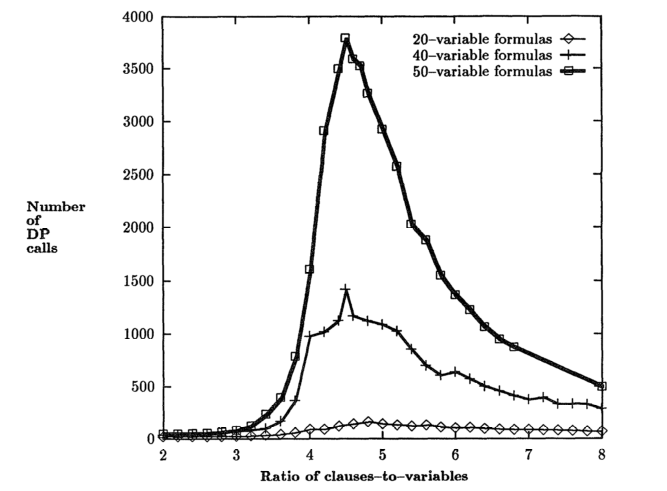
\includegraphics[width=1\textwidth]{Figures/GraphMitchellSelmanLevesque.png}
	\captionof{figure}{Median number of recursive DP calls for Random 3-SAT formulas, as a function of the ratio of clauses-to-variables. \\Extracted from Mitchell, Selman, and Levesque\cite{Mitchell}}
\end{center}
Therefore, an improvement of the input \emph{CNF} of the \emph{SAT Solver} can reduce a lot the hardness of the problem. \\
This is the main goal of the library, try to reduce the size of the final \emph{CNF} resulting from applying different converting methods on the original \emph{BF}.

%\section{Sate-of-art}


\section{Motivation}

\href{https://www.fib.upc.edu/en/studies/bachelors-degrees/bachelor-degree-informatics-engineering/curriculum/syllabus/LI}{Informatics Logic} is taught in this\footnote{\href{https://www.fib.upc.edu/en/}{Facultat Informàtica de Barcelona}} faculty. In that course I realized how important is \emph{logic} through its lecturer, \href{http://www.lsi.upc.es/~roberto/}{Dr. Robert Nieuwenhuis}, and its activities. \\

In the first coursework we had to code a \emph{SAT Solver} which used \emph{Unit Propagation}.
%\ref{A.2}. 
With this activity I comprehended how hard and substantial is the study of \emph{logic} and all its context. For example, how \emph{logic} is used in Artificial Intelligence and Planners.\\

When the time of deciding the \emph{TFG} arrived	, I contacted my actual supervisor, \href{https://www.cs.upc.edu/~jordicf/}{Dr. Jordi Cortadella}, and he proposed me some topics and ideas. Finally, we agreed on doing this project. \\

The motivation for this project is try to deepen into the topic and contribute on it.

\section{Stakeholders}

In this section the Stakeholders of the project are defined. Stakeholders are entities which are effected, directly or indirectly, by the solution developed in this project. 
\subsection{Target audience}
This tools tools targets all the entities (researchers, companies, \ldots) which works with \emph{PB minimization} and use \emph{SAT Solvers}.
\subsection{Users}
The users will be C++ programmers due this tool is developed in this language.
\subsection{Beneficiaries}
All those entities which works with \emph{PB minimization}. For example AI, SAT Solvers, Planners, \ldots



% Chapter Template

\chapter{Project Formulation} % Main chapter title

\label{Chapter1} % Change X to a consecutive number; for referencing this chapter elsewhere, use \ref{ChapterX}

%----------------------------------------------------------------------------------------
%	SECTION 1
%----------------------------------------------------------------------------------------

\section{Introduction}
\textcolor{red}{TODO
	There is an excellent introduction
	(context) that defines the terms
	and concepts of the subject under
	study. Stakeholders (target audience, users and beneficiaries)
	are fullyspecified.
	\\
	\\}

\textbf{Boolean satisfiability problems} \textit{(SAT from now on)} is the problem of finding a model\footnote{An interpretation which satisfies the formula.} for a boolean formula. In other words, it is the result of evaluating the boolean formula after replacing its variables for \emph{true} or \emph{false}. 
\\
SAT is widely used in Computer Science because it was the first problem proved to be NP-Complete\cite{Cook1971}\footnote{NP and NP-hard.} which allowed a lot of NP\footnote{Nondeterministic polynomial time.} to be reduced to it.

%-----------------------------------
%	SUBSECTION 2
%-----------------------------------

\subsection{What is First Order Logic?}
In propositional logic, a boolean formula is defined as following\cite{Lpo}:\\
Let $P$ be a set of predicate symbols like $p,q,r,...$
\begin{itemize}
	\item All predicate symbol of $P$ is a formula.
	\item If $F$ and $G$ are formulae, then $(F \land G)$ and $(F \lor G)$ are formulae to.
	\item If $F$ is a formula, then $(\neg F)$ is a formula.
	\item Nothing else is a formula.
\end{itemize}
This representation has some limitations because it can only express properties which are \emph{true} or \emph{false}.\\
This limitations can be overtaken using \textbf{First Order Logic} \textit{(FOL from now on)}. A FOL formula is defined as following\cite{Fol}:\\
\begin{itemize}
	\item text.
	\item text.
	\item text.
	\item text
\end{itemize}

%----------------------------------------------------------------------------------------
%	SUBSECTION 3
%----------------------------------------------------------------------------------------

\subsection{What is minimization?}

Sed ullamcorper quam eu nisl interdum at interdum enim egestas. Aliquam placerat justo sed lectus lobortis ut porta nisl porttitor. Vestibulum mi dolor, lacinia molestie gravida at, tempus vitae ligula. Donec eget quam sapien, in viverra eros. Donec pellentesque justo a massa fringilla non vestibulum metus vestibulum. Vestibulum in orci quis felis tempor lacinia. Vivamus ornare ultrices facilisis. Ut hendrerit volutpat vulputate. Morbi condimentum venenatis augue, id porta ipsum vulputate in. Curabitur luctus tempus justo. Vestibulum risus lectus, adipiscing nec condimentum quis, condimentum nec nisl. Aliquam dictum sagittis velit sed iaculis. Morbi tristique augue sit amet nulla pulvinar id facilisis ligula mollis. Nam elit libero, tincidunt ut aliquam at, molestie in quam. Aenean rhoncus vehicula hendrerit.
\chapter{Scope} % Main chapter title

\label{Chapter3} % Change X to a consecutive number; for referencing this chapter elsewhere, use \ref{ChapterX}

\section{What and how?}

Parlar del que es vol fer i com es fara
\\
requirements the project should meet\\
what to do? meet the requirements established by the client in particular, and by the rest of stakeholders



\chapter{Methodology and Rigor} % Main chapter title

\label{Chapter4} % Change X to a consecutive number; for referencing this chapter elsewhere, use \ref{ChapterX}

Research is a vast process with no clear path between \emph{a} and \emph{b}. For this, it is important to follow some directions. Methodology will provide some guidelines to avoid possible problems, be more efficient and do the project more manageable. 

\section{Methodology}
The methodology adopted for this project will be Agile\footnote{Methodology based on the on the adaptability in front of any change to improve exit possibilities.}. It is important to clarify that this methodology will not be followed strictly but adapted to this project where there is only one developer and all the objectives are well defined. The main characteristics followed from Agile in this project will be:
\begin{itemize}
	\item Short cycles
	\item TDD (Test-Driven Development)
	\item Weekly scrums with the supervisor
\end{itemize}

\section{Tools}
In this chapter the development tools for this project will be introduced. 
\subsection{Git}
\href{https://git-scm.com/}{Git} is a well known version control system developed by Linus Torvalds\footnote{Linux creator. \href{https://en.wikipedia.org/wiki/Linus_Torvalds}{(more)}}.\\
Git will be used in this project because it allows to maintain a tracking of all the changes made (commits), and what is more important, return to them at any time. In addition to this, it enforces a short cycle development (because commits are small units of work) and the developer has to document them which matches perfect with Agile methodology. 
\subsection{Trello}
\href{https://trello.com}{Trello} is a web board which helps to organize tasks and its state. It will be used for this project to define which tasks need to be done, its deadline and what its their current state. 
%\subsection{Mendeley}
%\subsection{CLion}

\section{Communication}
Due to my conditions, I'm currently studying abroad in an Erasmus program, all the communication will be made through electronic means. The majority of it will be made using e-mail but if it is necessary a video conference could be done. \\
The minimum communication with the supervisor will be a weekly e-mail report where all the tasks done during the week will be explained. Problems or questions will be also exposed, if any.

\section{Rigor and Validation}
Rigor and Validation for this project is relevant. \\
The surrounding of it, such as \emph{Artificial Intelligence, Planners, Cryptographic Protocols verification, \ldots}, are widely used nowadays and have been becoming more popular lately. This means that this project could have a big repercussion and be used by some professionals. For this, it is important to guarantee the validation and correctness of the project. \\
During the development, TDD will be used to avoid unnecessary code (possible origin of bugs) and assure the correctness of the implementation. It is also possible to formalize and prove all the operations done by the software.\\
Finally, my supervisor could give me orientation and validate, if necessary, the operations done.

%----------------------------------------------------------------------------------------
%	THESIS CONTENT - APPENDICES
%----------------------------------------------------------------------------------------

\appendix % Cue to tell LaTeX that the following "chapters" are Appendices

% Include the appendices of the thesis as separate files from the Appendices folder
% Uncomment the lines as you write the Appendices

% Appendix A

\chapter{Frequently Asked Questions} % Main appendix title

\label{AppendixA} % For referencing this appendix elsewhere, use \ref{AppendixA}

\section{How do I change the colors of links?}

The color of links can be changed to your liking using:

{\small\verb!\hypersetup{urlcolor=red}!}, or

{\small\verb!\hypersetup{citecolor=green}!}, or

{\small\verb!\hypersetup{allcolor=blue}!}.

\noindent If you want to completely hide the links, you can use:

{\small\verb!\hypersetup{allcolors=.}!}, or even better: 

{\small\verb!\hypersetup{hidelinks}!}.

\noindent If you want to have obvious links in the PDF but not the printed text, use:

{\small\verb!\hypersetup{colorlinks=false}!}.


%----------------------------------------------------------------------------------------
%	BIBLIOGRAPHY
%----------------------------------------------------------------------------------------
\printbibliography[heading=bibintoc]
%\addcontentsline{toc}{chapter}{Bibliography}

%----------------------------------------------------------------------------------------

\end{document}  
